\chapter{Future Work}
\label{sec:futurework}

This chapter will first introduce ideas for enhancing the CAL by further
adapters. Second, a design for multiple adapters within the CAL is discussed. Third, the
deployment of the developed system in existing simulation applications is examined.
Finally, ideas for load balancing and fault tolerance are presented. The discussed ideas
should be a guide for further development and call attention to the possibilities
of the GVON interface.

%%%%%%%%%%%%%%%%%%%%%%%%%%%%%%%%%%%%%%%%%%%%%%%%%%%%%%%%%%%%%%%%%%%%%%%%%%%%%%%%
%                                                                              %
% MORE ADAPTERS                                                                %
%                                                                              %
%%%%%%%%%%%%%%%%%%%%%%%%%%%%%%%%%%%%%%%%%%%%%%%%%%%%%%%%%%%%%%%%%%%%%%%%%%%%%%%%
\section*{Further Adapters}

The prototype implementation described in
Section~\ref{sec:implementation} utilized MPI as communication
back-end. While, MPI is probably available on every computing system
and implements probably every important communication protocol, other
interesting communication libraries could be used as communication
back-end.  This Section will discuss adapters based on a different
communication library than MPI.

% Internet Socket Based
\subsection*{Internet Socket Based Adapter}

Distributed applications, that are not deployed on clusters,
usually utilize different communication libraries to MPI. Two
interesting libraries are ZMQ and Boost Asio, which are both based
on the TCP/IP and UDP/IP protocol. They can be used to
interconnect applications over the internet. Therefore,
computations could be based on the internet as communication
network. Implementing an adapter for the CAL that interfaces with
ZMQ or Boost Asio would open an application based on the GVON interface
to the world of distributed computing over the internet.

Projects for distributed computing such as Folding@home
\cite{ref:folding_at_home} and SETI@home \cite{ref:seti_at_home},
utilize the computing power of computers distributed all over the
world connected via the internet.  These application distribute a
complex problem to a big number of peers. It would be interesting
to move an application from a cluster to a distributed environment
by just changing the CAL adapter (Figure~\ref{fig:internet_cal}).

\begin{figure}[H]
  \centering 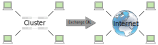
\includegraphics[width=\textwidth]{graphics/60_internet_cal}
  \caption{By exchanging the MPI adapter by an internet socket based
    adapter, an application previously executed on a cluster is also
    executable as an distributed application over the internet}
  \label{fig:internet_cal}
\end{figure}

\noindent A further use case is the connection of cluster nodes over
the internet. This would construct a grid computing environment based
on the GVON interface. This application could communicate via two CAL
objects, one local CAL configured by MPI and a global CAL
configured by internet sockets.  This approach could extend the
computational power of a cluster by further computing units of other
clusters.

% Adapters for Accelerators
\subsection*{Accelerator Based Adapter}

In contrast to the sender and receiver model of the communication over
a network such as the internet or a local area network, is the
communication with and in between accelerator devices mostly a
one-sided communication model.  An CAL adapter could model the offload
mechanism of accelerators for CUDA and OpenCL as communication
processes.

Since, offload is a one-sided communication concept, the
accelerator needs to be managed from a host CPU. This host
needs to transform the one-sided communication into a two-sided
communication that is supported by the developed system.

Therefore, Communication processes, such as send and receive,
between accelerators are managed by their hosts. In the world of the
developed system, the pair of host and device form a peer of the
CAL. Assume, two computers each equipped with an accelerator are
connected via a network. Transmitting data from one accelerator A to
another accelerator B (Figure~\ref{fig:acc_memcpy}) is separated into the following steps:

\begin{enumerate}
\item A Send data to B (send)
  \begin{enumerate}
  \item Copy of data from accelerator A memory to host A memory
  \item Sending of data to host B
  \end{enumerate}
\item B Receive data from A (recv)
  \begin{enumerate}
  \item Receiving of data from host A
  \item Copy of data from host B memory to accelerator B memory
  \end{enumerate}
\end{enumerate}

% MPI on CUDA devices
\noindent The adapter design for accelerators mentioned above has the
drawback that data has to take the detour above the host CPU. But, the
emerge of CUDA version 4.0 and 5.0 provides techniques that remove the
need of this detour. NVIDIA introduced with CUDA 4.0 the Unified
Virtual Addressing (UVA).  It creates a uniform address space of host
and devices of a single node. Utilizing UVA removes the need for
explicit copies from and to accelerators.

The introduction of further GPUDirect features with CUDA 5.0 offers
the possibility for direct exchange of data between accelerators on
the same node by P2P and of data between accelerator connected by a
network by RDMA.  Both approaches bypass the CPU and exchange data
directly over the PCI bus or network controller
(Figure~\ref{fig:gpudirect}).

\begin{figure}[H]
  \begin{minipage}[t]{0.5\textwidth} 
    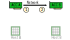
\includegraphics[width=\textwidth]{graphics/60_acc_memcpy}
    \caption{Exchanging data between accelerators. The data needs to be
    temporarily stored on the host memories until the data is
    transmitted over a network connection.}
    \label{fig:acc_memcpy}
  \end{minipage}%
  \begin{minipage}[t]{0.5\textwidth}
    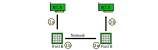
\includegraphics[width=\textwidth]{graphics/60_gpudirect}
    \caption{Direct exchange of data between accelerators over
      a network. The CPU memory is bypassed. NVIDIA provides such a
      technique by GPUDirect.}
    \label{fig:gpudirect}
  \end{minipage}%

\end{figure}


%%%%%%%%%%%%%%%%%%%%%%%%%%%%%%%%%%%%%%%%%%%%%%%%%%%%%%%%%%%%%%%%%%%%%%%%%%%%%%%%
%                                                                              %
% MULTIPLE ADAPTER                                                             %
%                                                                              %
%%%%%%%%%%%%%%%%%%%%%%%%%%%%%%%%%%%%%%%%%%%%%%%%%%%%%%%%%%%%%%%%%%%%%%%%%%%%%%%%
\section*{Multiple Adapter Design}
The possibility to exchange the adapter of the CAL also raises
the question if a design with more than one adapter at the same time
would be possible. Connecting the network of at least two adapters
would form a heterogeneous network, where each network provides 
properties like latency, bandwidth and hardware topology. The CAL
would unify these varying networks transparently under the same
interface. Thus, a multiple adapter design is the foundation for the
usage of the developed system in jungle computing environments (Section~\ref{sec:jungle}).

A CAL could be configured with an MPI adapter for communication inside
a cluster and with a internet socket adapter for communication over
the internet. This could connect two cluster systems over internet
to create a powerful tool to extend the computing power of a single
cluster.

Assuming a CAL configuration with two adapters mentioned above. Peers
that are present in the network of both adapters need to switch
between the adapters at run-time.  The CAL needs to provide a list of
all available adapters for a certain peer.  A particular sorting of
this list could state out the preferred adapter for communication
between two peers. Exchanging data between peers always requires a
look up of which adapter needs to be selected to address the
peers. The selection of a certain adapter can be performed at run-time
by a strategy pattern or partly at compile-time with variadic
templates.

Varying address spaces of the adapters have to be mapped onto the same
unified address space of the CAL.  This opens up the possibility that
two peers which do not share a same adapter, but are connected over a
third adapter, could still exchange data by routing over that third
adapter. Thus, a multiple adapter design does only make sense when
routing between two adapters is implemented.

Problems occur if collective operations are performed between varying
adapters. The collective operation has to be performed separately for
each adapter and then connected by a final collective operation.

Even if the design of a multiple adapter communication abstraction
layer looks quite interesting, the implementation is rather more
complex than a single adapter design. The decision for a single or
multiple adapter CAL should be placed in the hand of the application
developer.  Thus, the Cal could be configure by a further policy that
defines this adapter behavior.


%%%%%%%%%%%%%%%%%%%%%%%%%%%%%%%%%%%%%%%%%%%%%%%%%%%%%%%%%%%%%%%%%%%%%%%%%%%%%%%%
%                                                                              %
% DEPLOYMENT IN REAL WORLD SIMULATION                                          %
%                                                                              %
%%%%%%%%%%%%%%%%%%%%%%%%%%%%%%%%%%%%%%%%%%%%%%%%%%%%%%%%%%%%%%%%%%%%%%%%%%%%%%%%
\section*{Deployment in Real World Simulations}

Section~\ref{sec:impl:gol} and \ref{sec:impl:nbody} have shown that
implementations of Game of Life and N-body simulations on basis of the
GVON are possible. The performance evaluation in
Section~\ref{sec:eval:real} have shown no significant overhead in
respect to equivalent MPI implementations. Therefore, deploying the
developed system into real wold simulations would be the next step.

\subsection*{Deployment in PIConGPU}
In the beginning of this work, PIConGPU was the first simulation whose
communication processes were analyzed. But the system was not
developed for the sole objective of the utilization in
PIConGPU. Therefore, it was developed independently from PIConGPU.
The next step for evaluating the developed system is the deployment of
the GVON as library into PIConGPU. This will show how well the
developed system can be integrated into existing projects.

The PIConGPU communication processes are based on a three-dimensional
grid topology with diagonal connections. It does not differ to much
from communication patterns used in the GoL simulation. Thus, a
replacement of communication related parts in the PIConGPU source code
should be possible.

PIConGPU is interesting with respect of an accelerator based adapter
mentioned above, because calculations in PIConGPU are offloaded to
GPUs. Therefore, bypassing the CPU in case of accelerator to
accelerator communication would increase the overall performance.

% HASEonGPU
\subsection*{Deployment in HASEonGPU}
HASEonGPU is another project developed at the Helmholz Zentrum
Dresden Rossendorf (HZDR).  It was never an object of communication code
analyses, but it would be interesting if the developed communication
approach would fit on HASEonGPU.

HASEonGPU is a Monte-Carlo simulation of photons in a laser gain
medias. Whereby, the amplified spontaneous emission (ASE) of photons
is calculated for a set sample points in the simulated volume of
the gain media. The ASE value of each sample point can be calculated
independently from each other. Thus, a distribution onto a cluster
is possible.

A master peer distributes these set of sample points onto
available worker peers. This forms a communication based on a
star topology, where the master peer is placed as star center. In a
scenario with a lot of workload, e.g. by lot of sample points, the
master peer would be the communication bottleneck.

But, utilizing the GVON would provide the possibility to exchange this
topology. The star topology could be replaced by a more general tree
topology. The master peer could delegate the distribution task to
sub-master peers that are responsible for sub-trees of worker peers.
Figure~\ref{fig:haseongpu_topology} shows the graph representation of
both the star topology and the tree topology. 

\begin{figure}[H]
  \centering 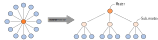
\includegraphics[width=\textwidth]{graphics/60_haseongpu_topology}
  \caption{The exchange of the present star topology by a tree topology
  leads to a better work distribution in scenarios with a lot of workload.}
  \label{fig:haseongpu_topology}
\end{figure}

\noindent The number of sub-master peers could be adapted by the
number of sample points.  Thus, more sample points increases the depth
of the tree topology which leads to a better workload distribution and
reduces the bottleneck effect.

%%%%%%%%%%%%%%%%%%%%%%%%%%%%%%%%%%%%%%%%%%%%%%%%%%%%%%%%%%%%%%%%%%%%%%%%%%%%%%%%
%                                                                              %
% GRAPH PARTITIONING                                                           %
%                                                                              %
%%%%%%%%%%%%%%%%%%%%%%%%%%%%%%%%%%%%%%%%%%%%%%%%%%%%%%%%%%%%%%%%%%%%%%%%%%%%%%%%
\section*{Load Balancing Ideas}

% Load balancing
In the beginning of this work it was clarified, that load balancing
will be not the focus of this work. Therefore, only rudimentary
distribution algorithms such round robin and consecutive distribution
were implemented. But, it was also claimed, that it should be possible
to build load balancing on top of the developed system.  The following
Sections will discuss ideas for load balancing based on the developed
system.

\subsection*{Graph Partitioning}

Assume, a simulation domain is modeled by a graph and the graph
contains more vertices than the number of peers in the global
context. These peers need to be oversubscribed by hosted vertices.
Therefore, the hosted vertices should be connected as close as
possible with respect to the graph. So that, communication of hosted
vertices of the same host are as local as possible.  This potentially
minimizes the number of messages that are transferred over the
network.

% Graph partitioning
A well researched solution for this problem is partitioning of
graphs. Partitioning divides the a graph into smaller partitions.  A
good partitioning algorithm reduces the number of edges running
between partitions.  Since the communication topology of the GVON is
described by a graph, this graph can be partitioned by already
existing graph partitioning tools.

% Metis
\subsection*{Metis - a Graph Partitioning Tool}
The tool METIS and its related tools hMETIS and ParMETIS are
established applications for graph partitioning. The developers claim
that they provide high quality partitions, are two magnitudes faster
than other widely used partitioning algorithms, and that graphs with
several millions of vertices can be partitioned in 256 parts in a few
seconds on current generation workstations and PCs.  The tool is
published under the Apache Licence Version 2.0., therefore, METIS
could support the graph distribution methods as library.
  
%%%%%%%%%%%%%%%%%%%%%%%%%%%%%%%%%%%%%%%%%%%%%%%%%%%%%%%%%%%%%%%%%%%%%%%%%%%%%%%%
%                                                                              %
% DESCRIPTION OF ADAPTER HARDWARE TOPOLOGY                                     %
%                                                                              %
%%%%%%%%%%%%%%%%%%%%%%%%%%%%%%%%%%%%%%%%%%%%%%%%%%%%%%%%%%%%%%%%%%%%%%%%%%%%%%%%
\subsection*{Description of the Adapter Hardware Topology}

% Cluster network topology
Cluster systems are equipped with varying network systems providing a
certain network topologies.  Utilizing the knowledge about the network
topology can increase application performance.  The most general
approach to describe the network topology of a cluster is a graph. A
network graph describes physical connections between nodes and could
be annotated with latency and bandwidth information.  This graph could
be the foundation of varying graph algorithm. For example could the
distance between two nodes be estimated and utilized to reduce
communication latency between peers.

With the existence of two graphs, one modeling the communication
topology of the simulation and another modeling the network
topology, a mapping between these graphs is possible.  Instead a
mapping from vertices to independent peers, vertices can be mapped
onto peers modeled in the network graph. Information that were used
to describe the network can be used to optimize this mapping.

In an oversubscribed case mention above, could the communication graph first be
partitioned to the number of available peers. After that, the
partitions will be mapped onto the peers.  An optimal mapping would
result in an graph homomorphism. Deciding whether there exists a
homomorphism from one graph to another, is NP-complete. Therefore, a
heuristically approach that tries to maximize the amount of same
adjacent vertices in communication and network graph should be
chosen. Figure~\ref{fig:graph_partitioning} shows a partitioning
of a graph and a mapping of these partitions onto peers.

\begin{figure}[H]
  \centering 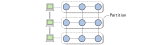
\includegraphics[width=\textwidth]{graphics/60_graph_partitioning}
  \caption{A two-dimensional grid is divided into three partitions.
    These partitions are mapped onto the available peers with respect
    to their network topology. Each peer is oversubscribed by three
    vertices.}
  \label{fig:graph_partitioning}
\end{figure}

% Load balancing
\noindent A Mapping between two graphs opens new possibilities for
load balancing.  The most simple load balancing approach is a load
balancing at the initialization of an application. The communication
graph is mapped only once and statically onto the network graph. This
approach is sufficient for applications that do not change with
respect to load distribution and graph topology.

But load distribution of simulations can change during run-time. The
difference in workload among peers could be estimated by run-time
measurements of a single time-step. The application needs to initiate
a rebalancing when the run-time of a host increases above a defined
threshold.

%%%%%%%%%%%%%%%%%%%%%%%%%%%%%%%%%%%%%%%%%%%%%%%%%%%%%%%%%%%%%%%%%%%%%%%%%%%%%%%%
%                                                                              %
% IDEAS FOR FAULT TOLERANCE                                                    %
%                                                                              %
%%%%%%%%%%%%%%%%%%%%%%%%%%%%%%%%%%%%%%%%%%%%%%%%%%%%%%%%%%%%%%%%%%%%%%%%%%%%%%%%
\section*{Fault Tolerance Ideas}

Similar to load balancing was fault tolerance of communication
processes not a topic for this work. Nevertheless offers the developed
system the possibility to build fault tolerance techniques on top.

The main problem of a simulation is the failure of a peer during
execution of simulation.  Some communication libraries such as MPI
have the embarrassing behavior that the whole program will fail
too. Therefore, the simulation has to be restarted, if only a single
peer fails.  Since, the amount of computing hardware increases with
each new cluster generation, it is not unlikely that a peer, that is
host for vertices of a simulation, fails. The library user has usually
no possibility to restart the failed peer, but the failed peer could
be replaced or even ignored in further communication processes.

% Reload from checkpoint
Assume, that each host checkpoints the state of its hosted
vertices at fixed points of the simulation execution. This
checkpoints could be written onto hard disk of an network attached
storage (NAS) or each host could distribute the data of its hosted
vertices to other host for backup reasons.

The network of hosts needs to notice the failure of hosts.
Furthermore, the hosts need to estimate where a failed host stored its
saved states.  Some host has to adopt the hosted vertices of
the failed host.  This so-called adopter host has to announce the
adopted vertices together with his already hosted vertices.  The
adopter host has to load the saved states of the adopted
vertices. In dependence whether the saved state is up-to-date,
other hosts also need to load their saved states. When all
vertices are synchronized to the same time-step, the communication and
therefore the simulation algorithm can be continued.


% Redundant calculations
Redistribute the hosted vertices of a failed host onto the remaining
host usually increases the workload each host has to manage.  Instead,
the vertices could be adopted by a backup peer that has no hosted
vertices so far.  Equally, to the previously mentioned method, needs
the backup peer to load the saved state from its adopted
vertices.

%%%%%%%%%%%%%%%%%%%%%%%%%%%%%%%%%%%%%%%%%%%%%%%%%%%%%%%%%%%%%%%%%%%%%%%%%%%%%%%%
%                                                                              %
% TWEAKS                                                                       %
%                                                                              %
%%%%%%%%%%%%%%%%%%%%%%%%%%%%%%%%%%%%%%%%%%%%%%%%%%%%%%%%%%%%%%%%%%%%%%%%%%%%%%%%
%\section*{Tweaks}
%
%\sitem{ Compile time generation of static graphs}
%\sitem{ Optimization of the graph to reduce overhead}
%\sitem{ Thread safe implementation of the gvon collectives}
%\sitem{ Multi-maps}


\cleardoublepage

%%% Local Variables:
%%% TeX-master: "diplom"
%%% End:
